\documentclass[border=10pt]{standalone}

\usepackage{tikz}
\usepackage{tikzsymbols}
\usetikzlibrary{calc,patterns,shapes.geometric}

\def\centerarc[#1](#2)(#3:#4:#5){\draw[#1] ($(#2)+({#5*cos(#3)},{#5*sin(#3)})$) arc (#3:#4:#5);}

\begin{document}
	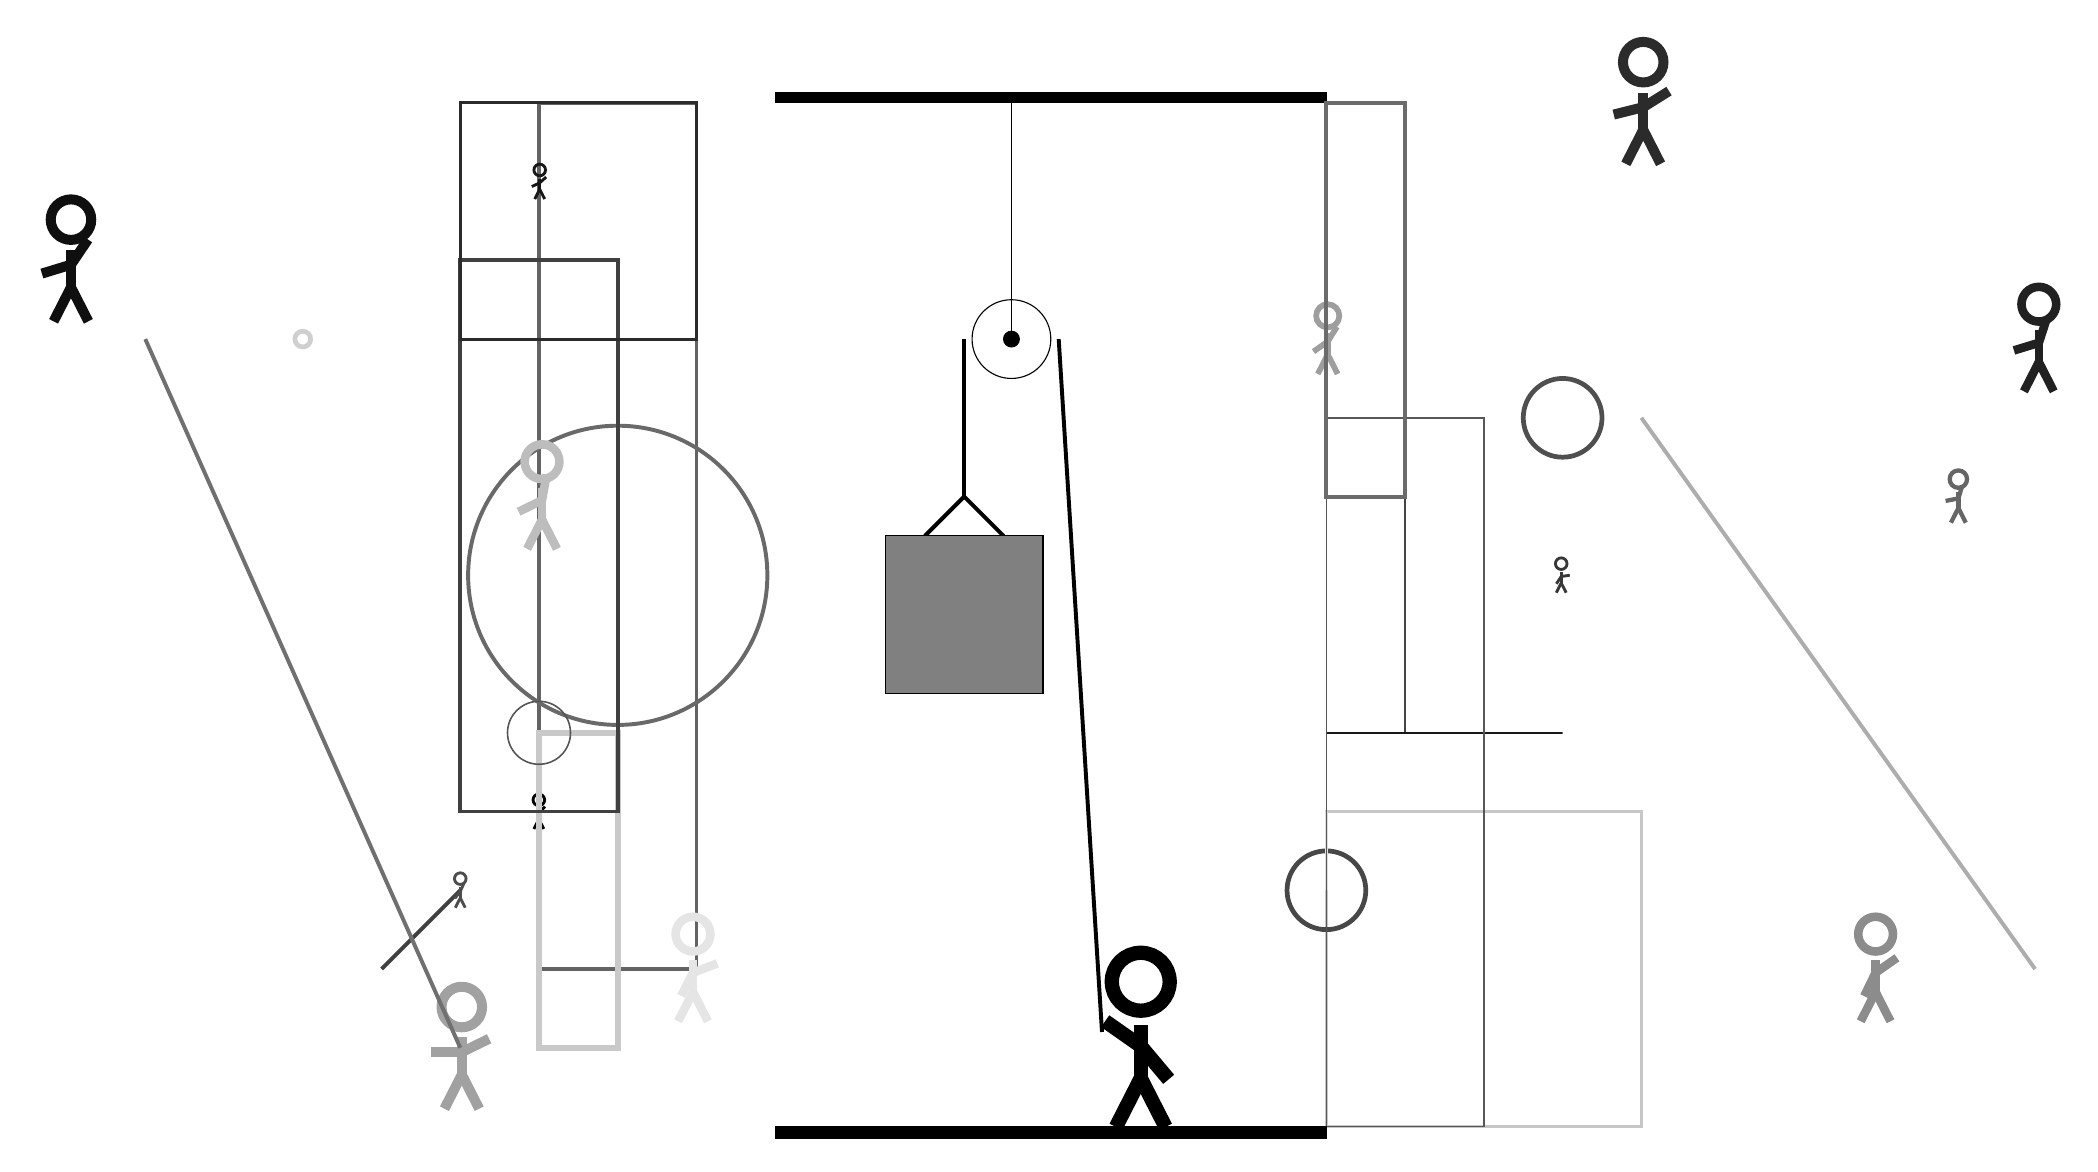
\begin{tikzpicture}
		%%%%% START %%%%%
		
		\draw[fill=black] (-2, 10) rectangle (5, 10.125);
		
		\draw (1, 7) circle (0.5);
		\draw[fill=black] (1, 7) circle (0.1);
		\draw (1, 10) -- (1, 7);
		
		\draw[line width=0.5mm, color=black!75](-6, 0) -- (-7, -1);
		
		\node[line width=0.7mm, color=black!38] at (5, 7) {\Strichmaxerl[4][35][58]};
		\node[line width=0.3mm, color=black!60] at (13, 5) {\Strichmaxerl[3][11][73]};
		\draw [line width=0.6mm, color=black!19](-8, 7) circle (0.1);
		\node[line width=0.3mm, color=black!37] at (-6, -2) {\Strichmaxerl[7][0][26]};
		
		\node[line width=0.2mm, color=black!99] at (-5, 1) {\Strichmaxerl[2][86][45]};
		
		\node[line width=0.4mm, color=black!87] at (14, 7) {\Strichmaxerl[6][17][72]};
		
		\node[line width=0.6mm, color=black!78] at (8, 4) {\Strichmaxerl[2][56][9]};
		\node[line width=0.5mm, color=black!94] at (-11, 8) {\Strichmaxerl[7][17][56]};
		\draw[line width=0.5mm, color=black!61] (-3, -1) rectangle (-5, 10);
		\draw [line width=0.5mm, color=black!59](-4, 4) circle (1.9);
		
		\node[line width=0.2mm, color=black!26] at (-5, 5) {\Strichmaxerl[6][26][80]};
		\node[line width=0.7mm, color=black!91] at (-5, 9) {\Strichmaxerl[2][25][42]};
		
		\draw[line width=0.5mm, color=black!32](9, 6) -- (14, -1);
		\draw[line width=0.7mm, color=black!21] (-4, 2) rectangle (-5, -2);
		\draw[line width=0.4mm, color=black!22] (5, -3) rectangle (9, 1);
		\draw [line width=0.6mm, color=black!72](5, 0) circle (0.5);
		\draw[line width=0.2mm, color=black!73] (6, 8) rectangle (6, 2);
		\draw[line width=0.3mm, color=black!90] (5, 2) rectangle (8, 2);
		\node[line width=0.5mm, color=black!83] at (9, 10) {\Strichmaxerl[7][14][32]};
		\draw[line width=0.5mm, color=black!75] (-4, 1) rectangle (-6, 8);
		\draw [line width=0.6mm, color=black!69](8, 6) circle (0.5);
		
		\node[line width=0.5mm, color=black!70] at (-6, 0) {\Strichmaxerl[2][52][66]};
		\draw[line width=0.4mm, color=black!13] (5, 0) rectangle (5, 1);
		\draw[line width=0.4mm, color=black!83] (-3, 7) rectangle (-6, 10);
		
		\node[line width=0.3mm, color=black!45] at (12, -1) {\Strichmaxerl[6][64][35]};
		\draw[line width=0.2mm, color=black!66] (5, 6) rectangle (7, -3);
		\draw[line width=0.5mm, color=black!58] (6, 10) rectangle (5, 5);
		\draw [line width=0.2mm, color=black!67](-5, 2) circle (0.4);
		\draw[line width=0.5mm, color=black!56](-6, -2) -- (-10, 7);
		\node[line width=0.3mm, color=black!10] at (-3, -1) {\Strichmaxerl[6][63][21]};
		
		\draw[line width=0.5mm] (-0.1, 4.5) -- (0.4, 5.0) -- (0.9, 4.5);
		\draw[fill=black!50] (-0.6, 4.5) rectangle (1.4, 2.5);
		
		\draw[line width=0.5mm] (0.4, 7) -- (0.4, 5.0);
		\centerarc[line width=0.5mm](1, 7)(0:180:0.6);
		\draw[line width=0.5mm](1.6, 7) -- (2.15, -1.8);
		
		\node at (2.6, -1.9) {\Strichmaxerl[10][-35][-50]};
		
		\draw[fill=black] (-2, -3) rectangle (5, -3.15);
		
		%%%%% END %%%%%
	\end{tikzpicture}
\end{document}